
\chapter{Symmetries and Conservation Laws}
\label{Symmetries}

We have first discussed symmetries and conservation laws when discussing about special relativity in Chapter~\ref{Relativity}. The reason for this is the intrinsic connection between relativity and the invariance of physical laws under translations in space and time. In this context we have discussed Noether's theorem and the links between symmetries and conservation laws.

The symmetries related to space-time are referred to as \emph{proper orthochronous Lorentz symmetries}, such as translation in time, translation and rotations in space. For each of them there is a corresponding conservation law, i.e.  conservation of energy, conservation of momentum and conservation of angular momentum. These transformations are called \emph{ proper} since they preserve the orientation in space, and \emph{orthochronous} because they preserve the orientation in time. 

We will discuss more symmetries here in the context of quantum mechanics. This will only be a very first taste of the fundamental concepts that will lead to \emph{gauge theories}, which play a central role in the description of interactions in quantum field theory. Before we start, it is worth pointing out that physical laws are not invariant under just any symmetry. 

We will briefly brush through the formalism of conserved quantities in quantum mechanics and discuss the different kinds of symmetries in nuclear and particle physics, trying to emphasise their role in making verifiable predictions. Our discussion will try to illustrate the distinction between the symmetries of space and time and \emph{internal symmetries} of a quantum mechanical system. To the proper orthochronous Lorentz symmetries we will add three symmetries of space and time. The first will be \emph{parity} (\(P\)) which is the inversion of space coordinates (or a point reflection) and is therefore not a \emph{ proper} transformation. We will also see the \emph{inversion in time} (\(T\)) which is not {\it orthochronous}. Then, we will see that there is a related symmetry which changes a particle into its anti-particle and is referred to as  \emph{charge conjugation} (\(C\)). The latter three symmetries are a bit different from the others, as they are \emph{discrete symmetries} and lead to multiplicative quantum numbers. 

In this chapter we will also detail other continuous symmetries, which are \emph{ internal} to a quantum mechanical system. A natural example of internal symmetries in quantum mechanics is the change of phase of a wave function,
\[ \psi \rightarrow \psi'= \psi e^{i\delta} \; \; \; \; {\rm where} \; \; \; \; |\psi'|^2 = |\psi|^2,\]
in which case all observable properties are invariant under such transformation.

A more detailed introduction to symmetries and conservation laws can be found in Chapter~10 of A. Das and T. Ferbel, ``Introduction to Nuclear and Particle Physics'', World Scientific\cite{DasFerbel}. Another excellent introduction to symmetries and conservation laws can be found in Richard Feynman's lectures~\cite{FeynmanSymmetries} which are always enlightening. 

The first and perhaps most striking symmetry observed at subatomic level is that as far as we can measure, particles (of a given fundamental type) are perfectly interchangeable. 

\section{Symmetries in quantum mechanics} \vskip 0.5cm

In Section~\ref{sec:Noether1} we have seen how invariance under  translations in space implied the conservation of momentum and the invariance under translations in time implied the conservation of energy. %These were the first two insights we have discussed of Noether's Theorem~\ref{TH:Noether}.

In quantum mechanics, the time evolution of an operator \(Q\) is given by
\[i \hslash \frac{dQ}{dt} =i\hslash \frac{\partial Q}{\partial t} + [Q,H].\]
Hence an operator which does not depend explicitly on time is conserved if it commutes with the hamiltonian \(H\):
\[ [Q,H]=0.\]
A transformation \(U\) doesn't affect \(H\) if 
\[UHU^{-1}=H,\]
so $UH=HU$ or $[U,H]=0$.

This is in the end a consequence of the requirement that physics predictions do not change after the transformation of the wave function
\[
\psi \to \psi'=U\psi.
\]
Physics predictions are the same whenever the normalisation of the wave function does not change under the transformation \(U\), which means requiring
\[
\langle\psi\mid\psi\rangle = \langle\psi'\mid\psi'\rangle
= \langle\psi U^\dag\mid U\psi\rangle,
\]
i.e. that
\[
U^\dag U=I,
\]
where we denoted the identity as $I$.

If $U$ is a continuous transformation, it may be imagined as a sequence of infinitesimal transformations, like in the case of spatial translations. These can be written as
\[
U(\epsilon) = I + i\epsilon \sigma,
\]
where $\epsilon$ is a real parameter which is infinitesimally close to zero, and $\sigma$ is called the \emph{generator} of the transformation. There is a requirement on $\sigma$ which comes from the fact that $U^\dag U=I$ should be satisfied:
\[
U(\epsilon)^\dag U(\epsilon) = (I-i\epsilon\sigma^\dag)(I+i\epsilon\sigma) = I + i\epsilon(\sigma - \sigma^\dag) + O(\epsilon^2),
\]
which means that one must have
\[
\sigma=\sigma^\dag,
\]
i.e.  $\sigma$ must be a hermitian operator, which commutes with the Hamiltonian as
\[
[H,U] = [H, I+i\epsilon\sigma] = 0,
\]
and hence it corresponds to a conserved quantity!

Moving to finite transformations is easy: we can see a finite transformation, which is a function of some parameter (or vector of parameters) $\alpha$, as a sequence of $n\rightarrow\infty$ infinitesimal transformations by $\epsilon=\alpha/n$, i.e. 
\[
U(\alpha) = \lim_{n\rightarrow\infty} \left(1+i\frac{\alpha}{n} \sigma\right)^n = \exp\left(i\alpha \sigma\right).
\]

In other words: for each symmetry of the Hamiltonian, there is an associated observed quantity $\sigma$.

%In general if U can be written as $e^{-i \epsilon \sigma}$ , where $\sigma$ is conserved. 

\section{Continuous symmetries}
Let's focus on the angular momentum. In the classic treatment it is intuitive how to combine two different angular momenta, while the task is far more complex in quantum mechanics.

The spin angular momentum does not come from a sum of components, because the electron for example can be considered an elementary particle. Spin is an intrinsic characteristic of elementary particles.

We can measure simultaneously the three components of a classical angular momentum, but in quantum mechanics we can measure simultaneously only the total amplitude $L^2$ and one of its components (typically $L_{z}$), and the resulting values are discrete.
$L^2$ can have eigenvalues $l(l+1)\hslash^2$ , where $l=0,1,2,3,\dots$ while the eigenvalues of $L_{z}$ will be $m_{l}\hslash$ , where $m_l=-l,-l+1,\dots,0,1,\dots,l-1,l$ , so $L_z$
 can assume $2l+1$ values. A given particle can have any angular momentum $l$, but its spin is fixed -- for example:
 \begin{itemize}
     \item \(S=0\): pions, kaons;
     \item \(S=\frac{1}{2}\): electron, muon, tauon, neutrinos, proton, neutron;
     \item \(S=1\): photon, some mesons, and the \(W\) and \(Z\) bosons;
     \item \(S=\frac{3}{2}\) - the $\Delta$ and $\Omega$ hadrons.
 \end{itemize}
Particles with an integer spin are called \emph{bosons}, and obey the Bose-Einstein statistics, while those with semi-integer spin are called \emph{fermions} and obey the Fermi statistics.

\subsection{Internal Symmetries}
We call \emph{internal symmetries} the symmetries which are not related to space and time, but rather on the relation between different particles. An example of internal symmetry is \emph{isospin}

\subsubsection{Composition of Angular Momenta}
When \(L\) and \(S\) are non-independent, the conserved quantity is the \emph{total} angular momentum
\[
\vec{J}=\vec{L}+\vec{S}.
\]
The question is how can we \emph{compose} angular momenta in quantum mechanics, as we cannot measure the three components simultaneously. 

Let us denote as \(\vec{J}_1\) and \(\vec{J}_2\) the two angular momenta to be composed.
The eigenvalues of the components along a given axis \(z\) can be summed directly,
\[
m=m_{1}+m_{2}
\]
The total amplitude of \(\vec{J}\) depends on the orientation of $\vec{J_{1}} $ and $\vec{J_{2}}$, and the possible values are
\[
j=|j_{1}-j_{2}|,|j_{1}-j_{2}|+1,\dots,|j_{1}+j_{2}|.
\]

Each state can be identified either in terms of \(j_1,m_1,j_2,m_2\), i.e. in terms of the eigenvalues of the two angular momenta being composed, or in terms of the eigenvalues \(j,m\) of the total angular momentum. 
The general expression to move from the former basis to the latter is
\begin{center}
      $|j_1 , m_1 \rangle |j_2 , m_2\rangle=\sum\limits_{j=|j_1-j_2|}^{j_{1}+j_{2}}c_{m,m_1 , m_2}^{j, j_1 j_2}|j,m\rangle$,
\end{center}
where the coefficients \(c\) of each state are the  \emph{Clebsh--Gordan coefficients}, which are tabulated (and whose derivation can be found in any quantum mechanics textbook). 

For example, one can compose a state with \(j_1=2,m_1=-1\) and another with \(j_1=1/2,j_2=1/2\), obtaining
\[\mid2 ,-1\rangle\mid\frac{1}{2} ,\frac{1}{2}\rangle=\sqrt{\frac{2}{5}}\mid\frac{5}{2} ,-\frac{1}{2} \rangle -\sqrt{\frac{3}{5}}\mid\frac{3}{2} ,-\frac{1}{2}\rangle,\]
where the coefficients are obtained from reading the horizontal lines of the Clebsh--Gordan tables in Fig. \ref{fig:clebsh1}.

\begin{figure}[h!]
\begin{center}
  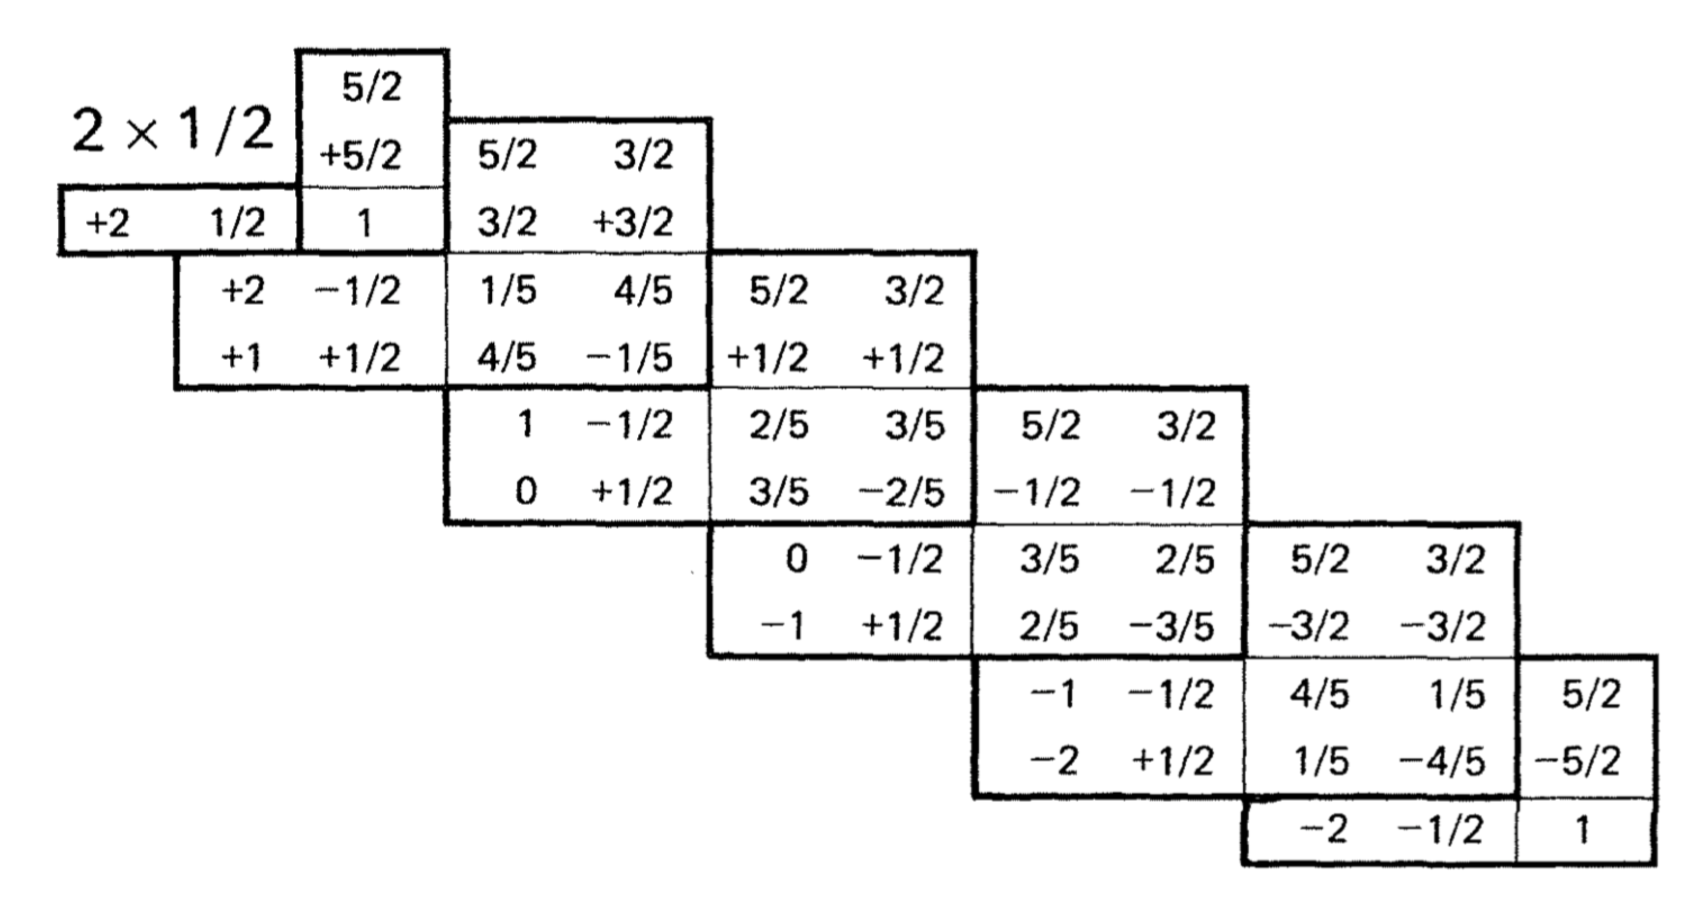
\includegraphics[width=10cm]{Figures/Simmetrie-pagine-1.pdf}\label{fig:clebsh1}
  \caption{Clebsh-Gordan table entries for the $2\times \frac{1}{2}$ composition}
\end{center}
\end{figure}

As for the decomposition of the states $\mid j,m\rangle$, one must read the tables vertically, obtaining
\[|j,m\rangle=\sum\limits_{j_1 , j_2}c_{m,m_1 , m_2}^{j, j_1 j_2}\mid j_1 , m_1 \rangle \mid j_2 , m_2\rangle.
\]

From the composition of two spins $\frac{1}{2}$ one can immediately observe the possible results:
\begin{itemize}
    \item total spin \(1\): a triplet state, symmetric under the exchange of particles;
    \item total spin \(0\): a singlet state, anti-symmetric under the exchange of particles.
\end{itemize}

In the case of a particle with spin $\frac{1}{2}$, a useful representation of the eigenstates \(\mid j, m\rangle \) is
\begin{align*}
\mid\frac{1}{2}   , \frac{1}{2}\rangle&=
\begin{pmatrix} 1\\ 0\\ 
\end{pmatrix}, \\
\mid \frac{1}{2} ,-\frac{1}{2}\rangle&=
\begin{pmatrix} 0\\ 1\\ 
\end{pmatrix},
\end{align*}
while a generic state of a particle with spin $\frac{1}{2}$ can be written as
\[
\alpha \begin{pmatrix} 1\\ 0\\ 
\end{pmatrix}+\beta \begin{pmatrix} 0\\ 1\\ 
\end{pmatrix}=\begin{pmatrix} \alpha\\ \beta\\ 
\end{pmatrix},
\]
where $\alpha$ and $\beta$ are complex numbers and $|\alpha|^2$ and $|\beta|^2$ are the probabilities of measuring $S_{z}=\frac{1}{2}\hslash$ and $S_{z}=-\frac{1}{2}\hslash$. Their sum is, of course, equal to one.

The choice of $S_{z}$ as a projection is arbitrary, so what are the probabilities of measuring $\frac{\hslash}{2}$ or $-\frac{\hslash}{2}$ on the other components? To each component of \(S\) is associated a matrix,
\begin{align*}
S_x &=\frac{ \hslash}{2}  \begin{pmatrix} 0& 1\\ 1&0\\
\end{pmatrix},\\
S_y &=\frac{ \hslash}{2}  \begin{pmatrix} 0& -i\\ i&0\\
\end{pmatrix},\\
S_z &=\frac{ \hslash}{2}  \begin{pmatrix} 1& 0\\ 0&1\\
\end{pmatrix}.
\end{align*}
Each matrix has eigenvalues $\pm \frac{ \hslash}{2}$. To find the probability of measuring a given value of $S_x$ it is sufficient to express $\begin{pmatrix} \alpha \\ \beta \\
\end{pmatrix}$ in the base of eigenvectors of $S_x$, and sum up the components:\par
\begin{center}
    $S^2=S_x^2+S_y^2+S_z^2$.
\end{center}
One must find $s(s+1)\hslash^2$ as a result.
The matrices (or \emph{operators}) $S_x$, $S_y$ and $S_z$ can be expressed using Pauli's matrices,
\[S_{x,y,z}=\frac{\hslash}{2}\sigma_{x,y,z}.\]

A rotation of the generic state $\begin{pmatrix} \alpha \\ \beta \\ 
\end{pmatrix}$ can be written as 
\[
\begin{pmatrix} \alpha' \\ \beta' \\ 
\end{pmatrix}=U(\vec{\theta})\begin{pmatrix} \alpha \\ \beta \\ 
\end{pmatrix},
\]
where $\vec{\theta}$ is a vector in the direction of the rotation and its amplitude is the angle of rotation. It is worth stressing that this is a rotation in the abstract Hilbert space, i.e. \emph{not} a rotation in space-time: in this transformation, all space-time coordinates are kept fixed.

A rotation in this space can also be represented as
\[
 U(\vec{\theta})=e^{-i \frac{\vec{\theta} \cdot \vec{\sigma}}{2}},
\]
where \(\vec{\sigma}=(\sigma_x,\sigma_y,\sigma_z)\) are the Pauli matrices. \footnote{Note that a rotation of spin is the exponential of a matrix, which is computed as
\[
e^A=1+A+\frac{1}{2}A^2+\dots +\frac{1}{n!}A^n+\dots.
\]}
The matrix $U(\vec{\theta})$ is unitary, has a determinant equal to \(1\) and the ensemble of these rotations is represented by the group of \(SU(2)\). The Pauli matrices are, in turn, the infinitesimal generators of \(SU(2)\).

One in general finds the following:
\begin{itemize}
    \item particles with spin $\frac{1}{2}$ are part of bi-dimensional representations of the group \(SU(2)\);
    \item particles with spin \(1\) are part of tri-dimensional representations of the group \(SU(2)\);
     \item particles with spin $\frac{3}{2}$ are part of tetra-dimensional representations of the group \(SU(2)\).
\end{itemize}

\subsubsection{Isospin}
From the point of view of strong interactions, replacing all protons with neutrons and vice-versa gives -- once Coulomb effects are subtracted -- the same results. It is then natural to consider the proton and the neutron as ``the same thing'', the nucleon, i.e. as parts of a doublet,
\begin{center}
   $ p=\begin{pmatrix} 1\\ 0\\ 
\end{pmatrix} $ \hskip 0.6 cm and \hskip 0.6cm $ n=\begin{pmatrix} 0\\ 1\\
\end{pmatrix} $.
\end{center}
Heisenberg proposed that strong interactions are invariant for rotations in the space of \emph{isospin}, whose name is in analogy with intrinsic spin.
This implies, thanks to  Noether's theorem, that the isospin is conserved in strong interactions.

We associate to particles which interact strongly (\emph{hadrons}) an isospin \(I\) and its projection $I_z$: we can form for example the proton-neutron doublet and the \(\pi\) meson triplet,
\[
    p=|\frac{1}{2},\frac{1}{2}\rangle,  \hskip 0.5cm
    n=|\frac{1}{2},-\frac{1}{2}\rangle, \hskip 0.5cm
    \pi^+=|1,1\rangle, \hskip 0.5cm
    \pi^0=|1,0\rangle, \hskip 0.5cm
    \pi^-=|1,-1,\rangle
\]
and also, for example,
\begin{itemize}
    \item particles with isospin 0: (spin $\frac{1}{2}$)\par
    $\Delta=|0,0\rangle$  
    \item particles with isospin $\frac{3}{2}$:(spin $\frac{3}{2}$)\par
    $\Delta^{++}=|\frac{3}{2},\frac{3}{2}\rangle$ \hskip 0.5cm
   $\Delta^{+}=|\frac{3}{2},\frac{1}{2}\rangle$ \hskip 0.5cm
    $\Delta^{0}=|\frac{3}{2},-\frac{1}{2}\rangle$ \hskip 0.5cm
     $\Delta^{-}=|\frac{3}{2},-\frac{3}{2}\rangle$
\end{itemize}
As in the case of spin, the multiplicity of each multiplet is \(2I+1\).

Isospin has a very important predictive power. Let's consider a system of two nucleons:  their possible configurations in terms of isospin are
\begin{itemize}
    \item triplet \par
  $  |1,1\rangle=pp \hskip 1cm
    |1,0\rangle=\frac{1}{\sqrt{2}}(pn+np) \hskip 1cm
     |1,-1\rangle=nn$
     \item singlet \par$
     |0,0\rangle=\frac{1}{\sqrt{2}}(pn-np) $ \hskip 1cm (Deuterium)
\end{itemize}
Since there are no bound states of two protons or neutrons, the solution to be chosen is the singlet,
So it seems that the strong attraction between nucleons is more important for \(I=0\) than for \(I=1\).

Isospin has implications in scattering reactions, let's consider
\begin{itemize}
    \item(i)\hskip 0.5cm p+p \begin{large} $\rightarrow$ \end{large} d + $\pi^+$,
    \item(ii)\hskip 0.45cm p+n \begin{large} $\rightarrow$ \end{large} d + $\pi^0$,
    \item(iii)\hskip 0.4 cm n+n \begin{large} $\rightarrow$ \end{large} d + $\pi^-$.
\end{itemize}
Considering that the deuteron has \(I=0\), we can write
\[
    d+\pi^+=|1,1\rangle, \hskip 1cm
    d+\pi^0=|1,0\rangle, \hskip 1cm
    d+\pi^-=|1,-1\rangle,
\]
while for the initial states we have\par
\begin{center}$
    p+p=|1,1\rangle, \hskip 1cm
    n+n=|1,-1\rangle, \hskip 1cm
   p+n=\frac{1}{\sqrt{2}}(|1,0\rangle+|0,0\rangle).
    $
\end{center}
Only the contribution \(I=1\) participates because the final state is $|1,0\rangle$ (and isospin is conserved in strong interactions), so the predicted amplitudes of scattering are in the ratios
\begin{center}
    $\mathcal{M}_{(i)}$\hskip 0.2cm:\hskip 0.2cm$\mathcal{M}_{(ii)}$\hskip 0.2cm:\hskip 0.2cm$\mathcal{M}_{(iii)}$\hskip 0.2cm=\hskip 0.2cm1\hskip 0.2cm:\hskip 0.2cm$\left(\frac{1}{\sqrt{2}}\right)$ \hskip 0.2cm:\hskip 0.2cm1,
\end{center}
so the cross sections are in the ratios
\begin{center}
$\sigma_{i}\hskip 0.2cm:\hskip 0.2cm\sigma_{ii}\hskip 0.2cm:\hskip 0.2cm
\sigma_{iii}\hskip 0.2cm=\hskip 0.2cm 2\hskip 0.2cm:\hskip 0.2cm 1 \hskip 0.2cm:\hskip 0.2cm 2 $
\end{center}
The processes (i) and (ii) have been measured ( (iii) is a bit more complex) ) and have been found in these proportions!

Another important example is the pion - nucleon scattering. Let's consider for example the three scattering processes
\begin{itemize}
    \item(i)\hskip 0.5cm $\pi^+ +p $ \begin{large} $\rightarrow$ \end{large} $\pi^+$ + p \hskip 1cm (elastic scattering),
    \item(ii)\hskip 0.45 cm $\pi^- +p $ \begin{large} $\rightarrow$ \end{large} $\pi^-$ + p \hskip 1cm (elastic scattering),
\item(iii)\hskip 0.4cm  $\pi^- +p $ \begin{large} $\rightarrow$ \end{large} $\pi^0$ + n \hskip 1cm (charge exchange).
\end{itemize}
We can write the initial and final states in terms of isospin states as
\begin{align*}
\pi^+ +p&=|1,1\rangle |\frac{1}{2}, \frac{1}{2}\rangle=|\frac{3}{2} ,\frac{3}{2}\rangle\\
\pi^- +p&=|1,-1\rangle |\frac{1}{2} \frac{1}{2}\rangle=\frac{1}{\sqrt{3}}|\frac{3}{2} ,-\frac{1}{2}\rangle-\sqrt{\frac{2}{3}}|\frac{1}{2}, -\frac{1}{2}\rangle\\
\pi^0 +n&=|1,0\rangle |\frac{1}{2} -\frac{1}{2}\rangle=\sqrt{\frac{2}{3}}|\frac{3}{2} ,-\frac{1}{2}\rangle+\frac{1}{\sqrt{3}}|\frac{1}{2}, -\frac{1}{2}\rangle.
\end{align*}
\begin{figure}[h!]
\begin{center}
  % Requires \usepackage{graphicx}
  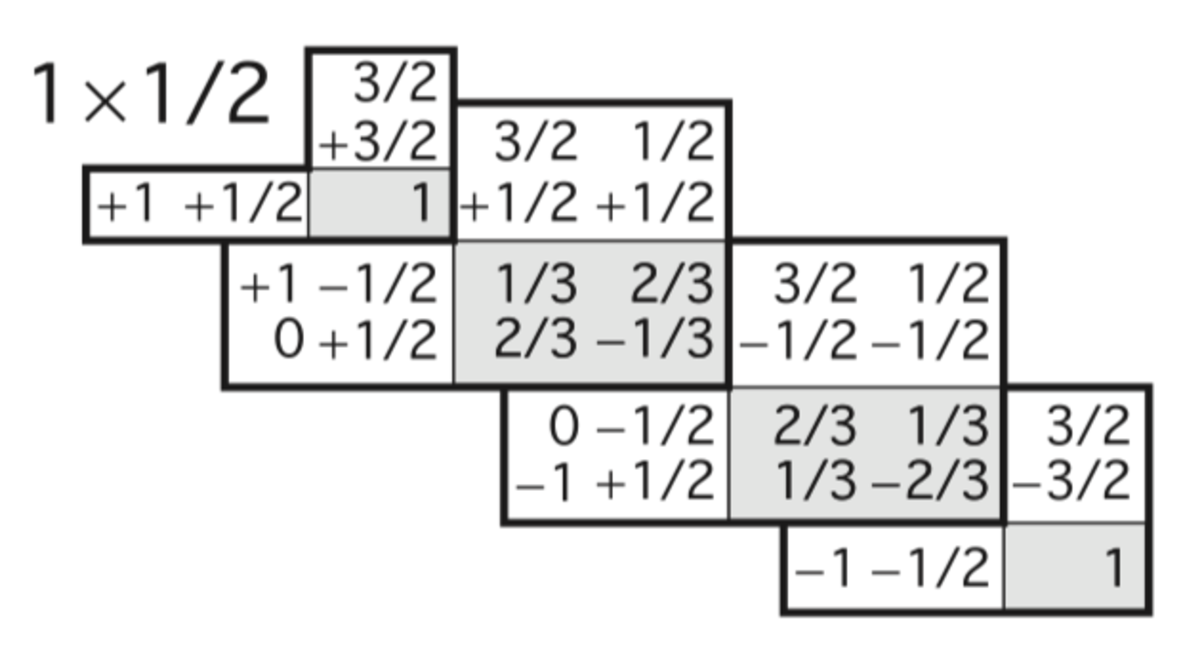
\includegraphics[width=8cm]{Figures/Simmetrie-pagine-2.pdf}\\
  \caption{Clebsch-Gordan tables for the $1\times\frac{1}{2}$ composition}
\end{center}
\end{figure}

In the case of nucleon-nucleon scattering yielding deuterium and a pion, there was only one possible value of total isopin, \(I=1\), so just one amplitude possible, and the proportions were fixed by the Clebsch-Gordan coefficients. In this case, instead, we have two different possible values for isospin, $I=\frac{3}{2}$ and $I=\frac{1}{2}$, so we consider two different amplitudes:
\begin{align*}
    \mathcal{M}_{3/2} \text{ for } I=\frac{3}{2} \qquad \langle I=\frac{3}{2}|H_{3/2}|I=\frac{3}{2}\rangle,\\
    \mathcal{M}_{1/2} \text{ for } I=\frac{1}{2} \qquad \langle I=\frac{1}{2}|H_{1/2}|I=\frac{1}{2}\rangle
\end{align*}
The first reaction (i) however has only a $I=\frac{3}{2}$ transition, and can be written as
\begin{align*}
    \pi^+ +p &\rightarrow \pi^+ +p,\\
    |\dfrac{3}{2} ,\dfrac{3}{2}\rangle &\rightarrow   |\frac{3}{2} ,\frac{3}{2}\rangle
\end{align*}
so
\[
\sigma_i =k|\mathcal{M}_{3/2}|^2.
\]
Similarly, for the reaction (ii):
\begin{align*}
    \pi^- +p &\rightarrow  \pi^- +p,\\
    \frac{1}{\sqrt{3}}|\frac{3}{2} ,-\frac{1}{2}\rangle-\sqrt{\frac{2}{3}}|\frac{1}{2}, -\frac{1}{2}\rangle&=|i\rangle=|f\rangle,
\end{align*}
which yields 
\[\sigma_{ii} =k|\frac{1}{3}\mathcal{M}_{3/2}+\frac{2}{3}\mathcal{M}_{1/2}|^2\]

While for reaction (iii),
\[\pi^- +p \rightarrow  \pi^0 +n,\]
we have:
\begin{align*}
    |i\rangle=\frac{1}{\sqrt{3}}|\frac{3}{2} ,-\frac{1}{2}\rangle-\sqrt{\frac{2}{3}}|\frac{1}{2}, -\frac{1}{2}\rangle,\\
    |f\rangle=\sqrt{\frac{2}{3}}|\frac{3}{2} ,-\frac{1}{2}\rangle+\frac{1}{\sqrt{3}}|\frac{1}{2}, -\frac{1}{2}\rangle
\end{align*}
so\[\sigma_{iii}=k|\sqrt{\frac{2}{9}}\mathcal{M}_{3/2}-\sqrt{\frac{2}{9}}\mathcal{M}_{1/2}|^2.\]

We can observe in collisions %discussione su acceleratori%  
    $\pi^- p $ and $\pi^+ p$ a resonance (Fig. \ref{fig:risonanzedelta}), given by the production of a $\Delta$ resonance with isospin $\frac{3}{2}$. This resonance appears at a mass of \SI{1232}{MeV}. It was empirically observed that $\mathcal{M}_{3/2}>>\mathcal{M}_{1/2}$, which allows to predict the ratios of cross sections to be
    \[
      \dfrac{\sigma_i}{\sigma_{ii}+\sigma_{iii}}=\dfrac{9}{1+2}.
    \]
  \begin{figure}[h!]
\begin{center}\label{fig:risonanzedelta}
  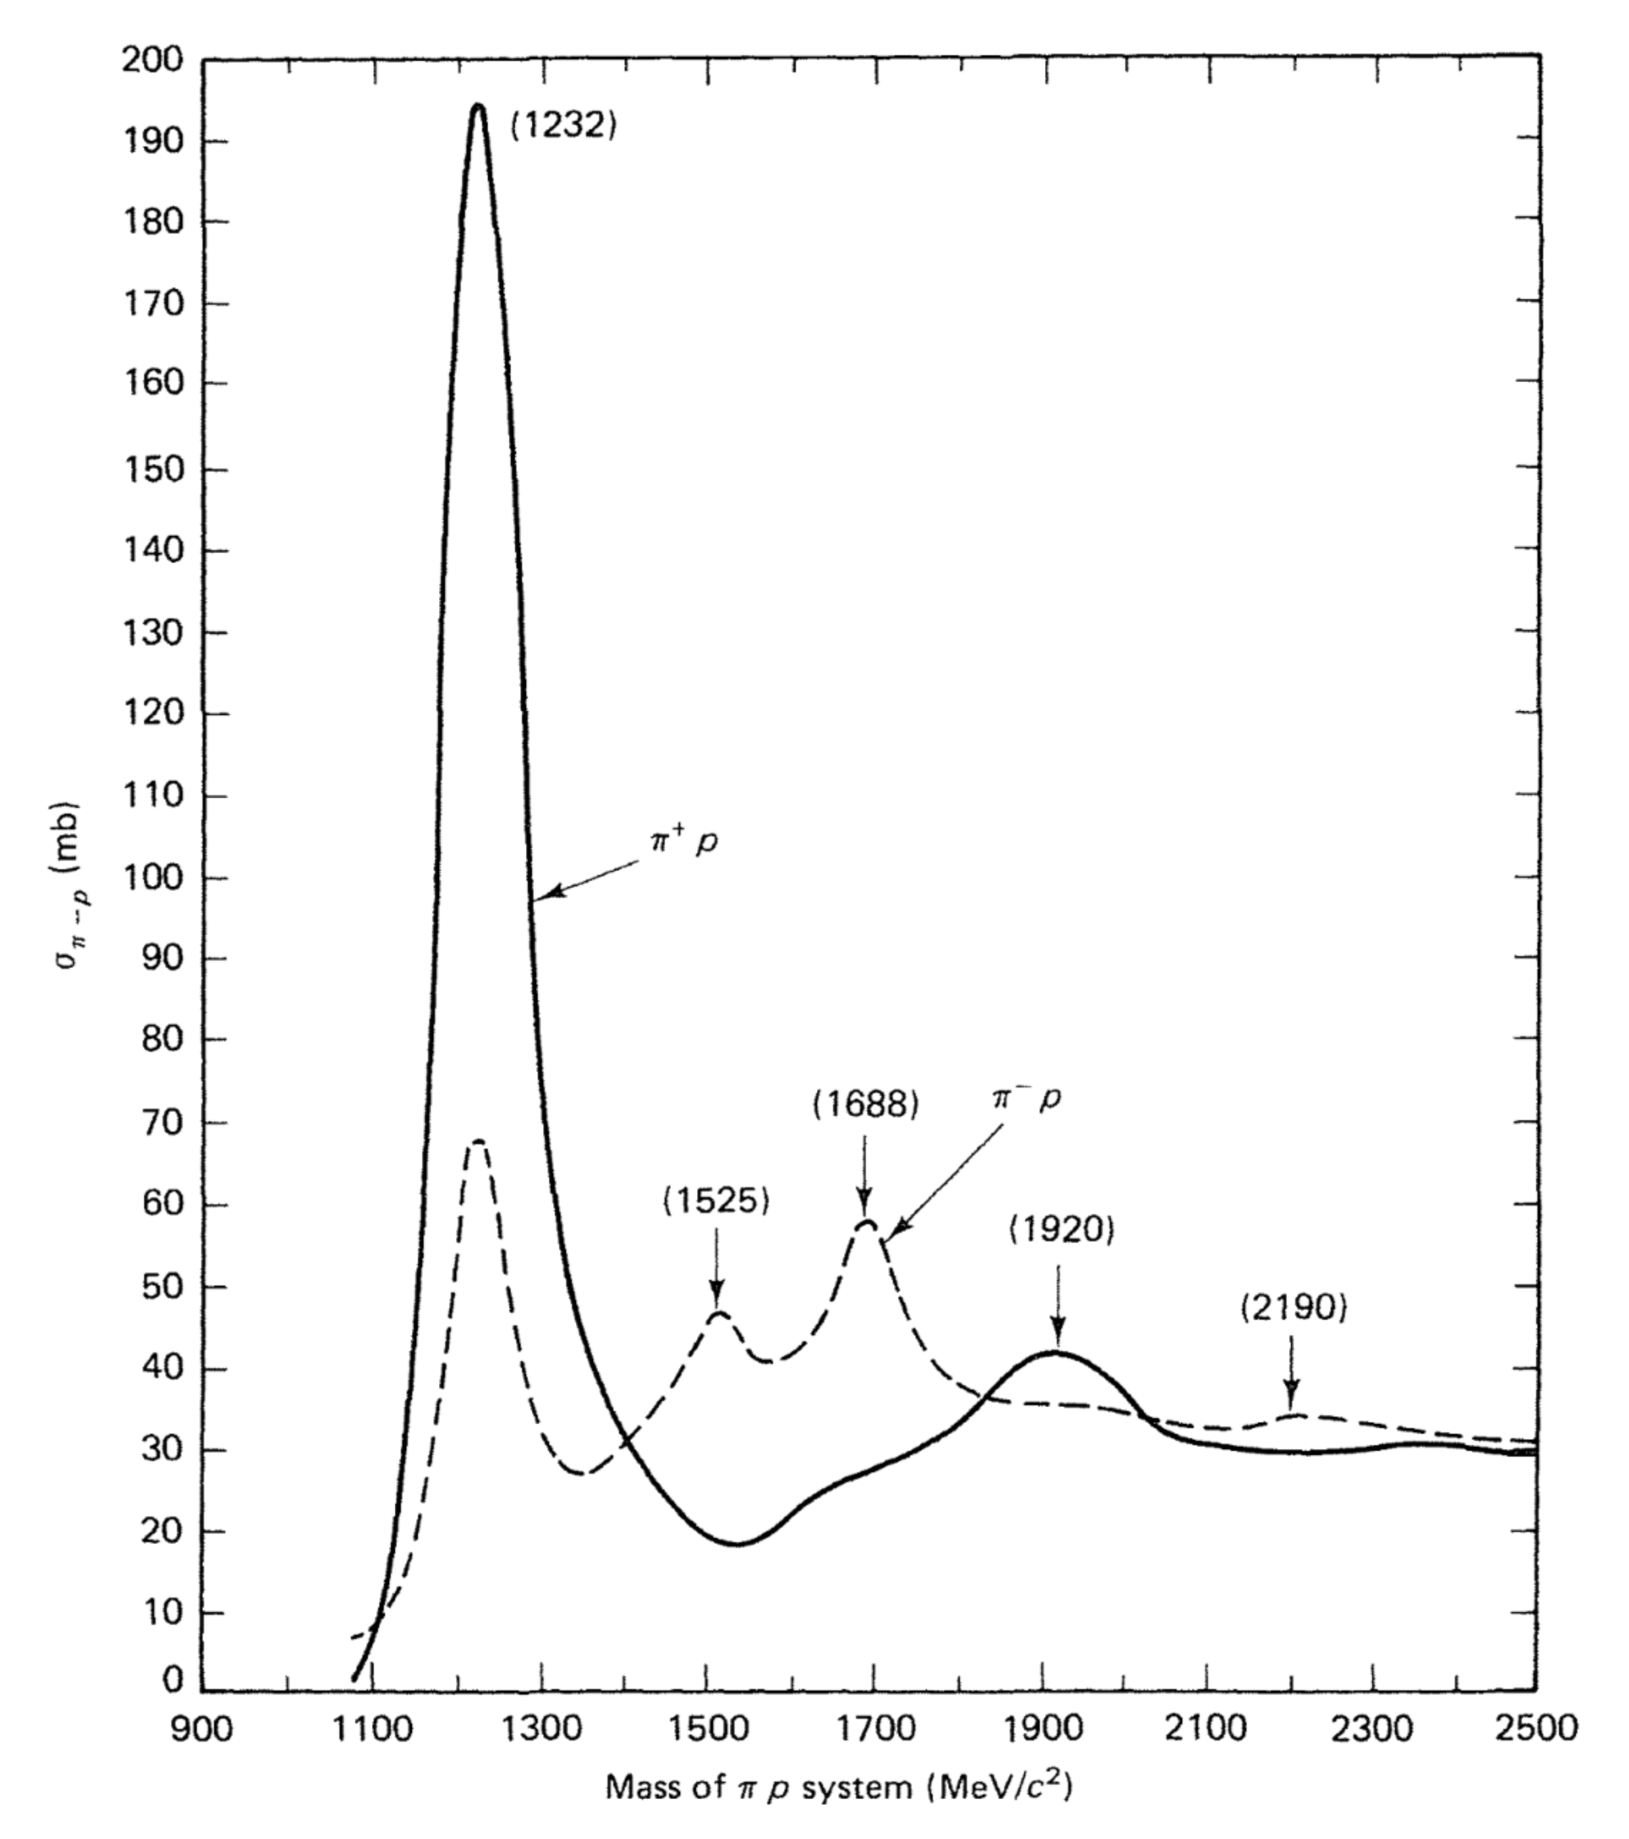
\includegraphics[width=12cm]{Figures/Simmetrie-pagine-3.pdf}\\
  \caption{Cross--section for \(\pi^\pm  p\) production as a function of the invariant mass.}
\end{center}
\end{figure}



\section{Discrete symmetries}
    In quantum mechanics there are various important discrete transformations:\par
    \begin{itemize}
        \item Parity P: \hskip 3cm$\vec{r}  \begin{large} \rightarrow \end{large} -\vec{r}$
        \item Charge-conjugation C:\hskip 1cm particle $ \begin{large} \rightarrow \end{large} $ antiparticle 
        \item Time reversal:\hskip 2.3cm$ t \begin{large} \rightarrow \end{large} -t$
    \end{itemize}\par
These transformations have the property that $P^2=T^2=C^2=1$ , so they are represented by operators with eigenvalues $\pm1$.

\subsection{Parity}
Vector quantities can have different types of parity, i.e. different behaviour after parity transformations:
\begin{itemize}
    \item \emph{polar vectors} are vectors that change sign with parity; for example,
    \begin{itemize}
        \item coordinates $\vec{r}$,
        \item velocity $\vec{v}$,
        \item momentum $\vec{p}$;
    \end{itemize}
    \item \emph{axial vectors} are vectors that do not change sign with parity; for example,
    \begin{itemize}
        \item angular momentum $\vec{L}=\vec{r}\land\vec{p}$,
        \item spin.
    \end{itemize}
\end{itemize}

Scalar quantities like $r^2, \frac{p^2}{2m}$, $L^2$,$\vec{L}\cdot\vec{S}$ do not change sign under parity transformations. Instead, dimension \(1\) quantities that \emph{do} change sign are called \emph{pseudo-scalars}.

Parity plays an important role in quantum mechanics. For a particle in a radial field, the wave function can be written in terms of harmonic functions,
\[\Psi_{n,l,m}=\frac{u_{n,l}}{r}Y_{l,m}(\theta,\phi),
\]
where the spherical harmonics $Y_{l,m}$ satisfy the relation
\[
P(\Psi_{n,l,m})=P(\frac{u_{n,l}}{r}Y_{l,m}(\theta,\phi))=\frac{u_{n,l}}{r}Y_{l,m}(\pi-\theta,\phi+\pi)=(-1)^l\Psi_{n,l,m}.\]
Assuming that the particle $\Psi$ has an intrinsic parity $R_{\Psi}$, then
\[
P\Psi_{n,l,m}=R_{\Psi}(-1)^l\Psi_{n,l,m}.
\]

In case of a system of two particles and an interaction with spherical symmetry, we have
\[
     P\Psi_{n,l,m}=R_{1}R_{2}(-1)^l\Psi_{n,l,m},
\]
i.e. the parity of a system of two particles with angular momentum \(l\) is given by
\[
P=P_1P_2(-1)^l,
\] where \(P_1\) and \(P_2\) are the intrinsic parities of the two particles.%Once we define the parity of a particle we can derive the others.

The electromagnetic interaction conserves parity. We can derive the parity of the photon by observing that:
\begin{itemize}
    \item $P(\vec{E})=-\vec{E}$ \hskip 1cm (i.e. the electric field is a polar vector),
    \item $P(\vec{B})=\vec{B}$ \hskip 1cm (i.e. the magnetic field is an axial vector).
\end{itemize}
The Maxwell equations are invariant under parity transformations, as
\begin{center}
    $\vec{\nabla}\cdot\vec{E}=\frac{\rho}{\epsilon_{0}}$ \hskip 2cm
     $\vec{\nabla}\land\vec{E}+\frac{\partial\vec{B}}{\partial t}=0$ \end{center}
    \hskip 2.8cm \begin{small} (-1)(-1)\hskip 0.3cm (1)\hskip 2cm (-1)(-1)\hskip 0.4cm (1) \par \end{small} \vskip 0.9cm
    \begin{center} $\vec{\nabla}\cdot\vec{B}=0$\hskip 2cm
        $\vec{\nabla}\land\vec{B}-\mu_{0}\epsilon_{0}\frac{\partial\vec{E}}{\partial t}=\mu_{0}\vec{J}$\end{center}
    \hskip 2.4cm  \begin{small}  (-1)(1)\hskip 2.6cm (-1)(1) \hskip 1cm (-1) \hskip 0.5cm (-1) \end{small}\par \vskip 0.7cm 
The interaction of the electromagnetic field has a polar nature, as
\[\vec{F}=(\vec{E}+\vec{v}\land\vec{B}).\]
Photons have spin one and negative parity: this can be seen, for example, from the fact that transitions between atomic levels with the emission of single photons have $\Delta l=\pm1$, which implies \(P(\gamma)=-1\).

Protons and neutrons are assigned positive parity,
\[P(p)=P(n)=+1.
\]
This is a convention analogous to the choice that the electron has a negative charge. Fermions $(e,n,p,\mu,\dots)$ have conventionally a positive parity, while their antiparticles have negative parity.

The parity of $\pi^-$ is measured from its capture at rest by the deuteron,
\begin{equation*}
   \pi^- +d \begin{large} \rightarrow \end{large} n+n.
  \end{equation*}
Experimentally this means sending a low-energy pion beam on a liquid deuterium target: pions are slowed down by energy loss, and then are captured in the atomic orbit to form a \emph{mesic atom} with \(d\).% The system decays rapidly, in a few \si{ps}, towards a principal quantum number state \(n=7\): the orbit of the pion overlaps with the deuteron nucleus, and the two interact via the strong force. This capture takes place with an angular momentum state of \(l=0\): since the spin of deuteron is \(1\) and the spin of the pion is \(0\), the initial state has \(J=1\). The deuteron is formed by two nucleons, i.e. by two fermions, with \(l=0\): therefore they have positive parity, and the initial parity of the system is equal to the intrinsic parity of the pion.
%The final state is composed by two identical fermions (the two neutrons), and therefore must be antisymmetric under the exchange of a neutron with the other. 

We know that the pion has spin $S_{\pi^{-}}=0$. As for the spin of deuterium, which is the bound state of a proton and a neutron: from the point of view of isospin\footnote{Which means: assuming that looking at the deuterium world without distinguishing between neutron and proton is correct. Or, more formally: assuming that isospin is a conserved symmetry -- which in reality isn't.}, its wavefunction should be antisymmetric under the exchange of nucleons; we have already seen that deuterium is an isospin singlet, so its isospin wavefunction is antisymmetric -- and hence, its spin and spatial wavefunctions should either be both antisymmetric, or both symmetric. The latter case is favoured by nuclear attraction, so we consider the ground state of deuterium the one with $S=1$ and $l=0$. As a consequence of this, in the initial state $J=1$ and the conservation of the total angular momentum implies that $J=1$ in the final state as well.

In order to know the parity of the pion in the initial state, we need to know the parity of deuterium and the spatial angular momentum of the initial state, $L_i$, which we can use to extract $P_{\pi^-}$ from
\[
P_i = (-1)^{L_i}\cdot P_{\pi^-} \cdot P_{d}.
\]
Since deuterium has $l=0$ and its constituents (the nucleons!) have positive parity, its parity will be $(-1)^0\cdot1\cdot1=1$. The initial state is in the S-wave, with the pion being captured by deuterium after having formed a so-called \emph{mesic} atom (where $d$ has the role of the nucleus and $\pi^-$ of the electron), so $L_i=0$. The missing piece of information is $P_i$, which we assume equal to the parity of the final state, $P_f$.\footnote{This is true only since this reaction happens though the strong force - we will see that parity isn't a conserved quantity in weak interactions.}

In order to calculate $P_f$, we need to know $L_f$ -- we know already $J$, so we just need to calculate $S_f$.
Since the final state has two identical fermions ($n$), Pauli's principle dictates that the final state must be anti-symmetric. What does it mean in terms of $S_f$?
\begin{itemize}
\item if $S_f=0$, we would have an antisymmetric spin wave function (singlet), so the spatial wave function would have to be symmetric, i.e. $L_f=0,2,\dots$ -- and having $J=L_f+S_f=1$ would be impossible!
\item if $S_f=1$, we would have a symmetric spin wave function (triplet), so the spatial wave function would have to be antisymmetric, i.e. $L_f=1,2\dots$ -- and this satisfies the requirement $J=L_f+S_f=1$ when $L_f=1$.
\end{itemize}
As a consequence of this, the final state (or initial state) parity can be written in terms of $L$ of the initial and final state (subscripts $i$ and $f$) and of the parity of neutrons (final state) and deuterium (initial state) as
\[
P_f=(-1)^{L_{f}}\cdot P_n \cdot P_n = P_i = (-1)^{L_i} \cdot P_{\pi^-} \cdot P_{d},
\]
or 
\[
P_f=(-1) \cdot (+1) \cdot (+1) = -1 = P_i = (+1) \cdot P_{\pi^-} \cdot (+1),
\]
i.e. the parity of $\pi^-$ is $-1$.

%so the spacial part given by the angular momentum must be of negative parity, so $P(\pi^-)=-1$
Since we do not observe the interaction $\pi^- d \rightarrow n n \pi^0$ , we can say that $P(\pi^0)=-1$.
The parity of $\pi^0$ can be measured directly in the decay:\par
\begin {center}
\begin{equation}
\pi^0  \begin{large} \rightarrow \end{large}e^+ + e^- + e^+ + e^-
\end{equation}
\end{center}
where each couple $e^+ e^-$ corresponds to an "inner photon" or a "virtual photon" , and the couples give the plane of polarization of the photons.\par
Parity is conserved in electromagnetic interactions, but it is not conserved in weak interactions, as it was discovered by Wu's experiment. 

\subsection{Charge Conjugation}
The transformation of \emph{charge conjugation} exchanges particles with their anti-particle:
\[ C(e^-)=e^+ \hskip 1cm C(e^+)=e^-.\]
Under this transformation, every quantum number is inverted; $C^2=1$, and the charge conjugation eigenvalues are $\pm1$. A few consequences follow:
\begin{itemize}
    \item charged particles cannot be eigenstates of \(C\);
    \item charge conjugation applied to a photon changes the sign of both the electric and the magnetic field, so $C(\gamma)=-1$;
    \item from the fact that the interaction $\pi^0 \rightarrow \gamma\gamma$ exists, we can deduce the relation
    \[
    C(\pi^0)=(C(\gamma))^2=1.
    \]
\end{itemize}
From this follows that the decay $\pi^0 \rightarrow \gamma\gamma\gamma$ is forbidden.

The charge conjugation is conserved in the strong interactions and in electromagnetic interactions, but not in the weak interactions.

\subsection{Time reversal}
Time reversal is a very interesting subject. We will neither discuss here the second law of thermodynamics, which states that the entropy of an isolated system cannot decrease with time, nor make any probabilistic considerations of configurations of an ensemble of particles in motion. We will focus on the reversibility in time of fundamental physical laws and concentrate on what happens under a very specific transformation, which is not quite as simple as just changing $t \rightarrow -t$.

In quantum mechanics, if we were to take the time reversal operator $T$ acting on a wave function $\ket{\psi(t)} = e^{-iHt/\hslash}\ket{\psi(0)}$ as:
\[T \ket{\psi(t)} = \ket{\psi(-t)} = e^{iHt/\hslash}\ket{\psi(0)},\]
then, since $T\ket{\psi(0)} = \ket{\psi(0)}$, we would have that
\[T \ket{\psi(-t)} =  e^{-iHt/\hslash}\ket{\psi(0)} =  e^{-iHt/\hslash} T \ket{\psi(0)},\]
which, given that $T\ket{\psi(-t)} = Te^{iHt/\hslash}\ket{\psi(0)}$, yields the relation
\[
e^{-iHt/\hslash} T =  T e^{iHt/\hslash}.
\]
Taking an infinitesimal change in time will then yield:
\[-i H T=  i T H.\]
This  means that such time reversal operator would not commute with the Hamiltonian, but instead would \emph{anti-commute}. As a consequence, for an energy eigenstate $\ket{E_n}$ one has
\[ H T \ket{E_n} = - TH \ket{E_n} = -E_n T \ket{E_n},\]
which implies that the $T$ operator would produce energies that could be indefinitely negative, and therefore the absence of a ground state. 

This can be avoided, by taking $T$ as an \emph{antilinear} operator, where an antilinear transformation $f: V \rightarrow V'$ from a complex vector space $V$ to another $V'$ is
\[f(a\vec{x} + b \vec{y}) = a^* f(\vec{x}) +b^* f(\vec{y})  \; \; \; \forall \; a, b \in \mathbb{C} \; \; {\rm and} \; \; \vec{x}, \vec{y} \in V.\]

As an antilinear operator, $T$,  will then act on the above wave function as
\[
   T(\psi(\vec{r},t)=\psi^*(\vec{r},-t).
\]
In this case, from the complex conjugate Schr\"{o}dinger's equation we have that
\begin{eqnarray*}
i\hslash \dfrac{\partial \psi(\vec{r},t)}{\partial t} &=&H\psi(\vec{r},t),\\
-i\hslash \dfrac{\partial \psi^*(\vec{r},t)}{\partial t}&=&H\psi^*(\vec{r},t), \\
i\hslash \dfrac{\partial \psi^*(\vec{r},-t)}{\partial t}&=&H\psi^*(\vec{r},-t), 
\end{eqnarray*}
so $\psi^*(\vec{r},-t)$ is still a solution of the Schr\"{o}edinger's equation with the same energies, if $THT^{-1}=H$.

\section{CPT Theorem}
The symmetries \(C\) and \(P\) are not fundamental symmetries of nature, as they are not conserved in weak interactions.
On the other hand one can demonstrate that any quantum field theory which
\begin{itemize}
    \item is invariant under Lorentz transformations;
    \item is local;
    \item has an hermitian hamiltonian;
\end{itemize}
must be invariant under the sequence (in any order!) of the three transformations \(CPT\).
As a consequence, particles and their antiparticles must have the same mass and the same lifetime.

\subsection{CP Violation in weak interactions}
TBA

\section{Summary of conservation laws}

Some fundamental symmetries can be related  to conservation laws through Noether's theorem:
\begin{itemize}
    \item Time translations - Energy conservation
    \item Space translation - Momentum conservation
    \item Rotations         - Angular momentum conservation
\end{itemize}

\begin{table}[]
    \centering
    \begin{tabular}{l|c|c|c}
    \hline \hline
        Quantum number & Strong Nuclear & Electromagnetic & Weak interaction \\ \hline
        \multicolumn{4}{c}{Continuous symmetries} \\ \hline
        Energy-momentum  & \checkmark & \checkmark & \checkmark  \\ \hline
        Electric charge  & \checkmark & \checkmark & \checkmark  \\ \hline
        Angular momentum  & \checkmark & \checkmark & \checkmark  \\ \hline
        Isospin   & \checkmark &   &   \\ \hline 
        Baryon number  & \checkmark & \checkmark & \checkmark  \\ \hline
        Lepton number  & \checkmark & \checkmark & \checkmark  \\ \hline
        Lepton flavor  & \checkmark & \checkmark & \checkmark  \\ \hline
        Strangeness  & \checkmark & \checkmark & $\Delta s =\pm 1$ \\ \hline
        Beauty  & \checkmark & \checkmark &   \\ \hline
 
         \multicolumn{4}{c}{Discrete symmetries} \\ \hline

        Parity (P) & \checkmark & \checkmark &   \\ \hline
        Charge conjugation (C) & \checkmark & \checkmark &  \\ \hline
        CP (or T)  & \checkmark & \checkmark &   \\ \hline
        CPT  & \checkmark & \checkmark &   \\ \hline \hline
    \end{tabular}
    \caption{Summary of conserved quantities relative to associated symmetries for the electromagnetic,  strong nuclear, and weak interactions.}
    \label{tab:my_label}
\end{table}

\section*{Take-home lessons}
\begin{itemize}
    \item Symmetries and conservation laws play a crucial role in fundamental physics. Symmetries are observed in nature and encoded in the mathematical description of physics; conservation laws arise as a consequence, through Noether's theorem.
    \item Invariance of physics laws by space translations implies the conservation of momentum, while invariance by time translations implies the conservation of energy. In quantum mechanics, quantities represented by operators are conserved if this operator commutes with the Hamiltonian.
    \item Angular momentum conservation is implied by rotational invariance. In quantum mechanics, one cannot simply sum angular momenta as in classical mechanics, but one rather applies composition laws (i.e. Clebsh-Gordan coefficients).
    \item Since the strong interaction seems to treat protons and neutrons in the same way, one may see atomic nuclei as composed by nucleons, and protons and neutrons as two different states of the nucleon. Isotopic spin, or \emph{isospin}, is introduced in analogy to spin. The same composition laws as angular momentum can be used to determine how probable it is for two strongly-interacting particles to interact together and produce two or more  particles, based on the intrinsic isospin of each of them.
    \item Symmetries which can be seen as a sequence of infinitesimal hermitian transformations are called \emph{continuous}. Symmetries which can't are called \emph{discrete}: for example, parity, charge-conjugation and time-reversal are all discrete transformations, with eigenvalues $\pm1$ (as applying them twice yields the same eigenstate).
    \item Parity ($P$) corresponds to flipping the sign of the spatial vector. Quantities are classified depending on how they transform under a parity transformation: for example, one may have polar vectors (which change sign after a parity transformation, e.g. position or momentum) and axial-vectors (which do not change sign, e.g. angular momentum and spin). The parity of a multi-particle system $C$ composed by two particles $A$ and $B$ is given by the product of the parity of the components, with a sign which depends on the total angular momentum of the system: $P_C=(-1)^{L_C}P_A P_B$.
    \item Charge conjugation ($C$) is the operation of flipping one particle with its anti-particle -- which has the same mass and spin of the original particle, but all other quantum numbers inverted (e.g. charge, isospin...).
    \item Time reversal $T$ does not simply correspond to changing $t$ with $-t$, as this would imply that the operator $T$ does not commute with the Hamiltonian, yielding the absence of a ground state in energy. Instead, time reversal is represented by an anti-linear operator, and the transformed wave function $T\psi$ is still a solution to the Schr\"odinger equation with the same energy as $\psi$.
    \item It is up to experiments to determine which interactions conserve which quantum numbers. Parity and charge conjugation  are conserved in electromagnetic and strong interactions, but are not in weak interactions; similarly, the sequence of $C$ and $P$ is conserved  in  electromagnetic and strong interactions, but not in weak interactions. The sequence of $C$, $P$ and $T$ is instead conserved by all interactions: this is a consequence of the \emph{CPT} theorem, which implies that particles and anti-particles have the same mass and mean lifetime.
\end{itemize}
\section*{Questions}
\begin{itemize}
    \item Weak interactions do not conserve strangeness. Does it mean that all processes mediated by the weak interaction imply a change of strangeness? Make an example.
    \item Make an example of pseudo-scalar quantity.
\end{itemize}